\documentclass[10pt]{article}

\usepackage{amsmath, amssymb, amsthm, newtxtext, physics}
\usepackage{graphicx}
\title{\textbf{Conformality and Invariance}}
\date{}
\usepackage[margins = 0.25in]{geometry}
\theoremstyle{plain} 
\newtheorem{definition}{Definition}
\newtheorem{theorem}{Theorem}
\newtheorem{example}{Example}
\newtheorem{observation}{Observation}
\newtheorem{proposition}{Proposition}
\begin{document}
	\maketitle 
	
\noindent \textbf{\textit{Goal:}} Define a notion of distance that is preserved under holomorphic \& conformal maps. Let's see why the regular notion of distance doesn't give us what we want.



\subsection*{The Jacobian of a Holomorphic Function}


Let $U \subseteq \mathbb{C}$ be an open set, $P \in U$ a fixed point, and $f: U \to \mathbb{C}$ a holomorphic function on $U$. For $f(x + iy) = u(x, y) + iv(x,y)$, we can consider $f$ as a mapping $(x, y) \to (u, v)$, where we get the real Jacobian matrix of $f$ at $P$: 
	\begin{eqnarray}
		J(P) = \begin{pmatrix}u_x(P) & u_y(P) \\ v_x(P) & v_y(P)\end{pmatrix}
	\end{eqnarray}
Since $f$ is holomorphic, by the Cauchy-Riemann equations we know that
	\begin{equation}
		\boxed{u_x = v_y, \qquad u_y = -v_x}
	\end{equation}
Hence, we can simplify (1) in the following way:
	\begin{align*}
		J(P) &=  \begin{pmatrix}u_x(P) & u_y(P) \\ v_x(P) & v_y(P)\end{pmatrix} \\
		&= \begin{pmatrix}u_x(P) & u_y(P) \\ -u_y(P) & u_x(P)\end{pmatrix} \\
		&= \underbrace{\sqrt{u_x(P)^2 + u_y(P)^2}}_{=: h(P)} \cdot \underbrace{ \begin{pmatrix} \frac{u_x(P)}{\sqrt{u_x(P)^2 + u_y(P)^2}} & \frac{u_y(P)}{\sqrt{u_x(P)^2 + u_y(P)^2}} \\ \frac{-u_y(P)}{\sqrt{u_x(P)^2 + u_y(P)^2}} & \frac{u_x(P)}{\sqrt{u_x(P)^2 + u_y(P)^2}} \end{pmatrix}} _{=: \mathcal{J}(P)}
	\end{align*}
Then, 
	\begin{equation}
		J(P) \equiv h(P) \cdot \mathcal{J(P)}.
	\end{equation}

We now make the following observations:
	\begin{observation} ~
		\begin{itemize}
			\item[(1)] $\mathcal{J}(P)$ is an orthogonal matrix.
			\item[(2)] The rows of $\mathcal{J}(P)$ form an orthonormal basis for $\mathbb{R}^2$ with positive orientation. 
			\item[(3)] For $\mathbf{x}, \mathbf{y} \in \mathbb{R}^2$, $$\norm{J(P) \mathbf{x} - J(P) \mathbf{y}} = h(P) \norm{\mathbf{x} - \mathbf{y}}.$$
			
			\item[(4)] If $\angle(\mathbf{x}, \mathbf{y})$ denotes the angle between two vectors $\mathbf{x}, \mathbf{y} \in \mathbb{R}^2$, then $$\angle (\mathbf{x}, \mathbf{y}) = \angle(J(P) \mathbf{x}, J(P) \mathbf{y}).$$
		\end{itemize}
	\end{observation}
	\begin{proof} ~
		\begin{itemize}
			\item[(1)] We have,
				\begin{align*}
					\left[\mathcal{J}(P) \cdot \mathcal{J}(P)^T\right]_{ij} &= [\mathcal{J}(P)]_{i1} [\mathcal{J}(P)^T]_{1j} + [\mathcal{J}(P)]_{i2} [\mathcal{J}(P)^T]_{2j} \\
					&= [\mathcal{J}(P)]_{i1} [\mathcal{J}(P)]_{j1} + [\mathcal{J}(P)]_{i2} [\mathcal{J}(P)]_{j2}
				\end{align*}
			So, by direct computation,
				\begin{align*}
					\left[\mathcal{J}(P) \cdot \mathcal{J}(P)^T\right]_{11} &= [\mathcal{J}(P)]_{11}^2 + [\mathcal{J}(P)]_{12}^2 \\
					&= \left(\frac{u_x(P)}{\sqrt{u_x(P)^2 + u_y(P)^2}}\right)^2 + \left(\frac{u_y(P)}{\sqrt{u_x(P)^2 + u_y(P)^2}}\right)^2 \\ \\
					&= \frac{u_x(P)^2}{u_x(P)^2 + u_y(P)^2} + \frac{u_y(P)^2}{u_x(P)^2 + u_y(P)^2} \\
					&= \frac{u_x(P)^2 + u_y(P)^2}{u_x(P)^2 + u_y(P)^2} \\
					&= 1 \\ 
					\\
					\left[\mathcal{J}(P) \cdot \mathcal{J}(P)^T\right]_{12} &= [\mathcal{J}(P)]_{11} \underbrace{[\mathcal{J}(P)]_{21}}_{= - [\mathcal{J}(P)]_{12}} + [\mathcal{J}(P)]_{12} \underbrace{[\mathcal{J}(P)]_{22}}_{= [\mathcal{J}(P)]_{11}} \\
					&= -[\mathcal{J(P)}]_{11} [\mathcal{J}(P)]_{12} + [\mathcal{J(P)}]_{11} [\mathcal{J}(P)]_{12} \\
					&= 0 \\
					\\
					\left[\mathcal{J}(P) \cdot \mathcal{J}(P)^T\right]_{21} &= [\mathcal{J}(P)]_{21} [\mathcal{J}(P)]_{11} + [\mathcal{J}(P)]_{22}[\mathcal{J}(P)]_{12} \\
					&= 0 \\
					\\
						\left[\mathcal{J}(P) \cdot \mathcal{J}(P)^T\right]_{22} &= [\mathcal{J}(P)]_{21}^2 + [\mathcal{J}(P)]_{22}^2 \\
						&= (-[\mathcal{J}(P)]_{12})^2 + [\mathcal{J}(P)]_{22}^2 \\
						&= 1.
				\end{align*}
		Hence, $$\mathcal{J}(P) \cdot \mathcal{J}(P)^T = \begin{pmatrix} 1 & 0 \\ 0 & 1\end{pmatrix}.$$
			\item[(2)] Just view the above computation, as we have shown that $$[\mathcal{J}(P)]_{11} [\mathcal{J}(P)]_{21} + [\mathcal{J}(P)]_{12} [\mathcal{J}(P)]_{22} = 0.$$ To show that the rows form an orthonormal basis with \textit{positive} orientation, we have
				\begin{align*}
					([\mathcal{J}(P)]_{11} \mathbf{i} + [\mathcal{J}(P)]_{12} \mathbf{j}) &\times ([\mathcal{J}(P)]_{21} \mathbf{i} + [\mathcal{J}(P)]_{22} \mathbf{j}) = \begin{vmatrix} [\mathcal{J}(P)]_{11} &  [\mathcal{J}(P)]_{12} \\  [\mathcal{J}(P)]_{21} & [\mathcal{J}(P)]_{22}\end{vmatrix} \mathbf{k} \\
					&= ([\mathcal{J}(P)]_{11} [\mathcal{J}(P)]_{22} - [\mathcal{J}(P)]_{12} [\mathcal{J}(P)]_{21})\mathbf{k} \\
					&= ([\mathcal{J}(P)]_{11}^2 + [\mathcal{J}(P)]_{12}^2) \mathbf{k}\\
					&= +\mathbf{k}
				\end{align*}
			
			\item[(3) - (4)] Since $\mathcal{J}(P)$ is an orthogonal matrix, it preserves lengths of vectors and angles between them, and thus (3) follows. A scaling transformation, which is what $h(P)$ is, obviously preserves angles, and so (4) follows. 
		\end{itemize}
	\end{proof}

\subsection*{Conformal Mappings of the Unit Disk}
\noindent Since the author of this book says that\textbf{\textit{ conformal mappings}} are characterized by the fact that they infinitesimally 
	\begin{itemize}
		\item[(i)] preserve angles, and
		\item[(ii)] preserve length (up to a scalar factor) 
	\end{itemize}
we have just shown that
	\begin{theorem}
		The Jacobian $J(P)$ of a holomorphic map $f: U \subseteq \mathbb{C} \to \mathbb{C}$ at a point $P \in U$ is a conformal map. 
	\end{theorem}
\noindent 
	Despite this, $J(P)$ fails to preserve distances. So we have an example of a conformal map that doesn't preserve Euclidean distance. Let's reduce our view to conformal mappings of the unit disk for the time being. 

	When $U$ is the unit disk in $\mathbb{C}$, we have a nice classification theorem for all conformal mappings on $U$. 
	
	\begin{theorem}[The Conformal Mappings of the Unit Disk]
		Let $D = D(0, 1)$ denote the unit disk in $\mathbb{C}$. Then a conformal mapping on $D$ is either
			\begin{itemize}
				\item[(i)] A rotation $\rho_\lambda : z \mapsto e^{i \lambda} \cdot z$, $0 \leq \lambda < 2 \pi$;
				
				\item[(ii)] A Möbius transformation of the form $\varphi_a : z \mapsto [z - a]/[1 - \overline{a} z]$, $a \in \mathbb{C}$, $|a| < 1$; or 
				
				\item[(iii)] A composition of mappings of type (i) and (ii).
			\end{itemize}
	\end{theorem}

\subsection*{Constructing the Poincaré Metric}
To "discover" the Poincaré metric, we start with what we want (invariance of the metric under conformal mappings) and go from there. 
	\begin{enumerate}
		\item Given any vector, sourcing from a point $P$ in the direction of $\mathbf{v}$, denote its \textit{length} by $|\mathbf{v}|_P$. 
		
		\item Declare that the length of $\mathbf{e} = (1, 0)$ is 1. So, $|\mathbf{e}|_0 = 1$. 
		
		\item If $\phi$ is a conformal self-map of the disk, then we claim that the condition
			\begin{equation}
				|\mathbf{v}|_P = |\phi_\ast(P) \mathbf{v}|_{\phi(P)},
			\end{equation}
		where $\phi_\ast(P)\mathbf{v} := \phi'(P) \cdot \mathbf{v}$ denotes the \textit{\textbf{push-forward}} by $\phi$ of the vector $\mathbf{v}$, is equivalent to invariance under this new metric we're defining. Why? Since $\phi'(P)$ is the Jacobian of $\phi$ at $P$, then by our previous work, this action amounts to a rotation and a scaling. We're saying the above condition encapsulates that, after that rotation and scaling, the length of our vector stays the same. Now, we are \textit{requiring} that $|\cdot|$ is such that (4) works for any conformal self-map of the disk $\phi$. We're using this condition to derive an explicit formula for $|\cdot|$.
		
		
		\item Let $\phi(z) = e^{i \lambda} \cdot z$. Then, first of all $$\phi(z) = (\cos \lambda + i \sin \lambda)(x + iy) = x \cos \lambda  - y \sin \lambda + i (x \sin \lambda + y \cos \lambda)$$ so then, 
			$$\phi'(z) = \begin{bmatrix} \cos \lambda & -\sin \lambda \\ \sin \lambda & \cos \lambda \end{bmatrix}$$  
		Condition (4) says that we must have $$1 = |\mathbf{e}|_0 = |\phi_\ast(0) \mathbf{e}|_{\phi(0)} = |e^{i \lambda} \cdot \mathbf{e}|_0 = |e^{i \lambda}|_0$$ Therefore, we conclude the length of any Euclidean unit vector based at the origin is 1 in this new invariant metric.
		
		\item Let $\phi(z)$ be the Möbius transformation $$\psi(z) = \frac{z + a}{1 + \overline{a} z}$$ with $a \in \mathbb{C}$, $|a| < 1$. Let $\mathbf{v} = e^{i \lambda}$ be a unit vector at the origin. Then, with $$\psi'(0) = 1 - |a|^2$$ and (4), we have $$1 = |\mathbf{v}|_0 = |\psi_\ast(0) \mathbf{v}|_{\psi(0)} = |(1 - |a|^2) \cdot \mathbf{v}|_a$$ Hence, $$|\mathbf{v}|_a = \frac{1}{1 - |a|^2}.$$
		We are ready.
	\end{enumerate}

	\begin{definition}[The Poincaré Metric]
		Let $P$ be a point of the unit disk $D$ and let $\mathbf{v}$ be any vector based at that point. Then, $$\boxed{|\mathbf{v}|_P = \frac{\norm{\mathbf{v}}}{1 - |P|^2}}$$ is called the \textbf{\textit{Poincaré metric}}. 
	\end{definition}

	\noindent Note that, with the above definition, as $P$ approaches $\partial D$, my ramen noodles get cold. Just kidding. Actually, $|\mathbf{v}|_P \to \infty$ is what happens, but at the same time my ramen noodles do indeed get cold.
	
	
	What does space "look like" if you were living under the Poincaré metric? With regards to Definition 1, simply look at the image of $D$ under the map $$f(x, y) = \frac{1}{1 - |x^2 + y^2|}, \qquad x^2 + y^2 < 1.$$ As in Figure 1 above. 
	
		\begin{figure}
			\centering
			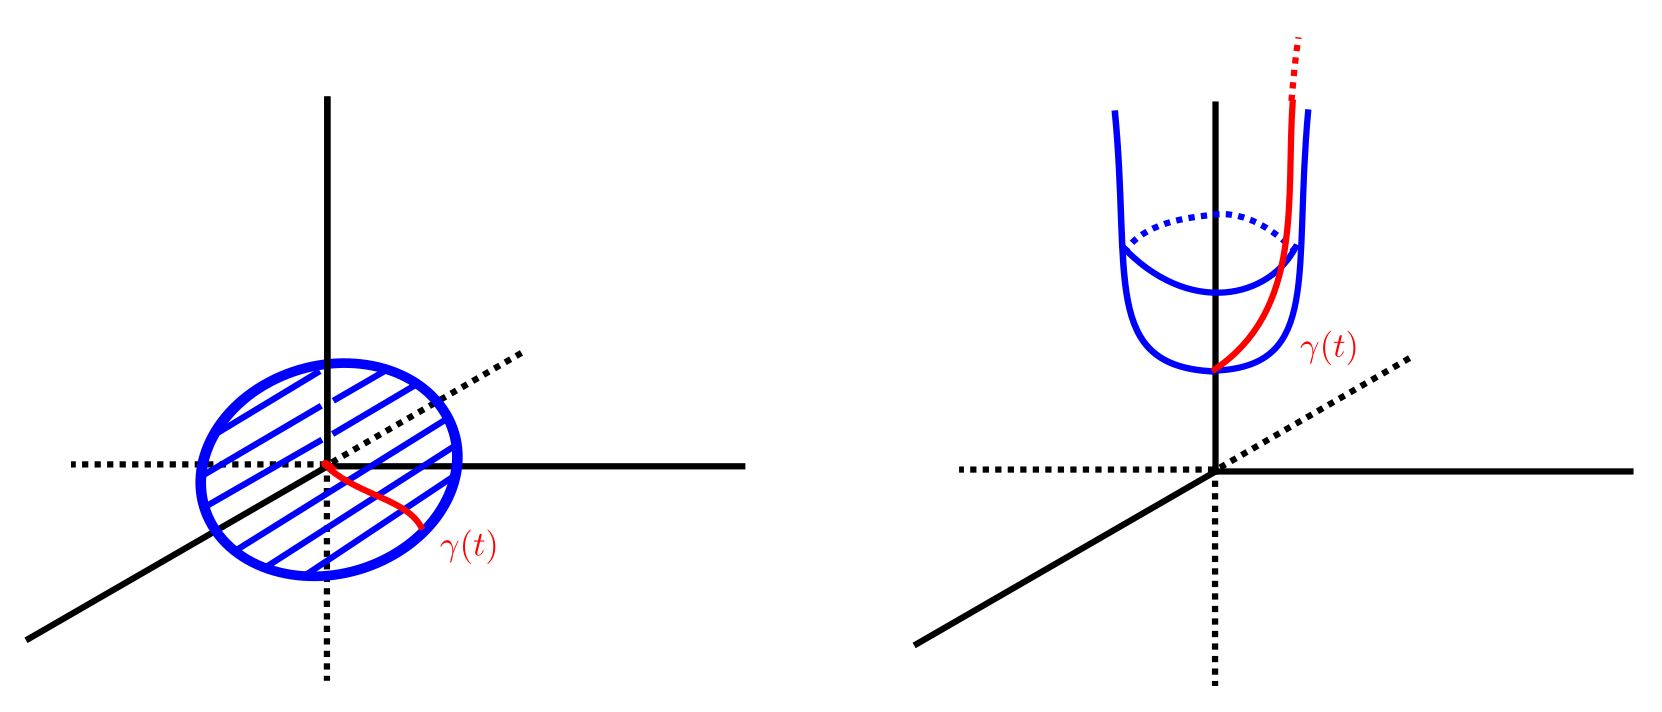
\includegraphics[scale = 0.25]{images/pcmetric.JPG}
			\caption{\small{A visualization of how the Poincaré metric warps distances. On the left is the disk $D = \{(x, y) : x^2 + y^2 < 1\}$ and on the right is the image of that disk under the map $f(x, y) = \frac{1}{1 - |x^2 + y^2|}.$ Note that when working with the Poincaré metric, we don't "see" this surface. We are like an ant living on it and can only observe the effects. To us, it is like we are still living on a disk, but the distance between two points on the disk is different: take $p_0 = \mathbf{0}$, the origin, and take a point $p$ on $\gamma(t)$ close to $\partial D$. When the disk is equipped with the standard Euclidean metric, the distance between $p_0$ and such $p$ is bounded above by 1. With the Poincaré metric, as $f$ has a ring asymptote for $(x, y)$ close to $\partial D$, the distance between $p$ and $p_0$ becomes unbounded.}} 
		\end{figure}
	We now define the length of a curve under the Poincaré metric using geodesics. 
		\begin{definition}
			Let $\gamma: [0, 1] \to D$ be a continuously differentiable curve. The \textbf{\textit{length}} of $\gamma$ in the Poincaré metric is given by $$\ell(\gamma) = \int_0^1 |\gamma'(t)|_{\gamma(t)} \ dt = \int_0^1 \frac{\norm{\gamma'(t)}}{1 - |\gamma(t)|} \ dt.$$ 
		\end{definition} 
	
		\begin{example}
			Let $\epsilon > 0$ and consider the curve $\gamma(t) = (1 - \epsilon)t$, $0 \leq t \leq 1$. Then, the length of $\gamma$ is given by
				\begin{align*}
					\ell(\gamma) &= \int_0^1 |\gamma'(t)|_{\gamma(t)} = \int_0^1 \frac{(1 - \epsilon)}{1 - |\gamma(t)|^2} \ dt \\
					&= \int_0^1 \frac{(1 - \epsilon)}{1 - [(1 - \epsilon)t]^2} \ dt = \frac{1}{2}\int_{u(0)}^{u(1)} \frac{du}{1 - u} \qquad u = (1 - \epsilon)t^2 \\ 
					&=  \frac{1}{2} \left[\log \left(\abs{\frac{u(1) + 1}{u(1) - 1}}\right) - \log\left(\abs{\frac{u(0) - 1}{u(0) + 1}}\right)\right] = \frac{1}{2}\left[ \log\left(\frac{2 - \epsilon}{\epsilon}\right) - \log\left(\abs{\frac{-1}{1}}\right) \right]\\
					&= \frac{1}{2} \log \left(\frac{2 - \epsilon}{\epsilon}\right)
				\end{align*} 
			
		\end{example}
		
		The use of this example is to give a computational understanding of Figure 1. As $\epsilon \to 0^+$, $\ell(\gamma) \to +\infty$. As $\epsilon \to 0^+$, $\ell(\gamma)$ is becoming the line connecting $0$ to the boundary point $(\cos(\pi/4), \sin(\pi/4))$, in some sense, the distance from 0 to the boundary (along this linear path) is infinite. 
		
		\begin{definition}
			Let $P, Q \in D$. Then, the \textbf{\textit{Poincaré distance}} $d(P, Q)$ between $P$ and $Q$ is given by $$d(P, Q) = \inf_{\gamma \in E} \ell(\gamma)$$ where $E$ is the collection of all piecewise continuously differentiable curves connecting $P$ to $Q$. (Note that the length of a piecewise differentiable curve is the sum of the lengths of its continuously differentiable pieces.)
		\end{definition}
		\begin{proposition} ~
				\begin{itemize}
					\item[(1)] The disk $D$ equipped with the Poincaré distance $d(\cdot, \cdot)$ is a metric space. 
					
					\item[(2)] Let $P \in D$. Then, the Poincaré distance of $0$ to $P$ is equal to $$d(0, P) = \frac{1}{2} \cdot \log \frac{1 + |P|}{1 - |P|}.$$
				\end{itemize}
		\end{proposition}
		\begin{proof} ~
			\begin{itemize}
				\item[(1)] ~
					\begin{itemize}
						\item ($d(x, x) = 0$) Let $x \in D$. By definition 2, first take note that $$0 \leq \ell(\gamma) = \int_0^1 \frac{\norm{\gamma'(t)}}{1 - |\gamma(t)|} \ dt.$$ Now, $\gamma(t) \equiv_{t \in [0, 1]} x$ is a continuously differentiable curve connecting $x$ to itself, we have $$\ell(\gamma) = \int_0^1 \frac{0}{1 - x} \ dt = 0$$ and it follows that $d(x, x) = 0$.
						
						\item ($d(x, y) > 0$) Let $x, y \in D$ by distinct points. Suppose for contradiction that $d(x, y) = 0$ so that $$\inf \ell(\gamma) = 0.$$ Therefore, there exist $\gamma_1, \gamma_2, \gamma_3, \dots$ connecting $x$ and $y$ such that $\ell(\gamma_1) \geq \ell(\gamma_2) \geq \ell(\gamma_3) \geq \cdots$ and $$\lim_{n \to \infty} \ell(\gamma_n) =  \lim_{n \to \infty} \int_0^1 \frac{\norm{\gamma_n'(t)}}{1 - |\gamma_n(t)|} \ dt= 0.$$ For now, suppose that the $\gamma_1, \gamma_2, \dots$ are continuously differentiable. By the mean value theorem for vector-valued functions\footnote{See \textit{Principles of Mathematical Analysis} (3rd edition) by Walter Rudin, p. 113, Theorem 5.19}, for each $n = 1, 2, 3 \dots$, there exists $c \in (0, 1)$ such that $$|\gamma(1) - \gamma(0)| \leq (1 - 0)\norm{\gamma_n'(c)} \implies |y - x| \leq \norm{\gamma_n'(c)}.$$  Since $\lim_{n \to \infty} \ell(\gamma_n) = 0$, it follows that as $n \to \infty$, $\ell(\gamma_n') \to 0$ and hence $|y - x| = 0$, a contradiction to our presupposition that they are distinct. Now, what if the curves in the sequence $\gamma_1, \gamma_2, \gamma_3 \dots$ are piecewise continuously differentiable? Without loss of generality, suppose $\gamma_1, \gamma_2, \gamma_3$ are all continuously differentiable on the same segments $\{I_m = (a_m, a_{m + 1})\}_{m = 1}^N$ with $a_1 = 0$ and $a_{N + 1} = 1$ (we can say w.l.o.g. because we can start with $\gamma_1$ and re-parameterize $\gamma_2, \gamma_3, \dots$ to be continuously differentiable on the same intervals that $\gamma_1$ is), and so $$\ell(\gamma_n) = \sum_{m = 1}^N \int_{a_m}^{a_{m + 1}} \frac{\norm{\gamma_n'(t)}}{1 - |\gamma_n(t)|} \ dt.$$ Since all constituent parts of the sum are positive, and we know that $\lim_{n \to \infty} \ell(\gamma_n) = 0$, it follows that for all $m = 1, 2, \dots, N$, $$\lim_{n \to \infty} \int_{a_m}^{a_{m + 1}} \frac{\norm{\gamma_n'(t)}}{1 - |\gamma'(t)|} \ dt = 0.$$ Applying the same analysis as above, gives that $\lim_{n \to \infty} \gamma(a_m) = \lim_{n \to \infty} \gamma(a_{m + 1})$ for all $m = 1, 2, \dots, N$, giving $$ \lim_{n \to \infty} \gamma(a_1) = \lim_{n \to \infty} \gamma(a_{N + 1}) \implies y = x$$ which is a contradiction.  
						
						\item (Triangle inequality) Let $x, y, z \in D$ be distinct.  
					\end{itemize}
				
				\item[(2)]
			\end{itemize}
		\end{proof}
\end{document}